\documentclass[12pt,a4paper,twoside,openright,final]{memoir}
\usepackage{fontspec}
\usepackage{amsmath}
\usepackage{amsfonts}
\usepackage{amssymb}
\usepackage{makeidx}
\usepackage{graphicx}
\usepackage[hidelinks,unicode=true]{hyperref}
\usepackage[spanish,es-nodecimaldot,es-lcroman,es-tabla,es-noshorthands]{babel}
\unaccentedoperators
\usepackage[left=3cm,right=2cm, bottom=4cm]{geometry}
\usepackage[sort&compress]{natbib}
\usepackage{microtype}
\usepackage{extras/tfm}
\usepackage{ifdraft}
\usepackage[obeyDraft]{todonotes}
\ifdraft{
	\usepackage{draftwatermark}
	\SetWatermarkText{BORRADOR}
	\SetWatermarkScale{0.7}
	\SetWatermarkColor{red}
}{}
\usepackage{booktabs}
\usepackage{longtable}
\usepackage{calc}
\usepackage{array}
\usepackage{subcaption}
\usepackage{footnote}
\usepackage{minted}
\usetikzlibrary{spy}

\setsansfont[Ligatures=TeX]{texgyreadventor}
\setmonofont{FreeMono}

\newfontfamily\myfont{FreeMono}


\defaultfontfeatures{}

\newfontfamily\noligsmonofamily[NFSSFamily=noligsmonofamily]{FreeMono}


\author{José Ignacio Escribano}

\usepackage{amsmath}
\usepackage{xparse}
\usepackage{amsthm}
\usepackage{tikz}

% Seno
\def\sen{\mathop{\mbox{\normalfont sen}}\nolimits}

% Seno hiperbólico
\def\senh{\mathop{\mbox{\normalfont senh}}\nolimits}

% Arcoseno
\def\arcsen{\mathop{\mbox{\normalfont arcsen}}\nolimits}

% Gradiente
\def\grad{\mathop{\mbox{\normalfont grad}}\nolimits}

% Argumento principal
\def\Arg{\mathop{\mbox{\normalfont Arg}}\nolimits}

% Logaritmo complejo
\def\Log{\mathop{\mbox{\normalfont Log}}\nolimits}

% Rotacional
\def\rot{\mathop{\mbox{\normalfont rot}}\nolimits}

% Divergencia
\def\diver{\mathop{\mbox{\normalfont div}}\nolimits}

% Longitud
\def\longi{\mathop{\mbox{\normalfont long}}\nolimits}

% Índice de una curva
\def\ind{\mathop{\mbox{\normalfont Ind}}\nolimits}

% Rango de una matriz
\def\rang{\mathop{\mbox{\normalfont rang}}\nolimits}

% Norma
\newcommand{\norm}[1]{\lVert #1 \rVert}

% Derivada parcial
\newcommand{\derpar}[1]{\dfrac{\partial}{\partial #1}}

% Derivada parcial con función
\newcommand{\derparcial}[2]{\dfrac{\partial #1}{\partial #2}}

% Derivada parcial de orden n con funcion
\newcommand{\derparcialn}[3]{\dfrac{\partial^{#3} #1}{\partial #2^{#3}}}

% Integral doble en [a,b] x [c,d]
\newcommand{\intdob}[4]{\displaystyle \int_{#1}^{#2} \int_{#3}^{#4}}

% Integral triple en [a,b] x [c,d] x [e,f]
\newcommand{\inttri}[6]{\displaystyle \int_{#1}^{#2} \int_{#3}^{#4} \int_{#5}^{#6}}

% Números complejos
\def\C{\ensuremath{\mathbb{C}}}

% Números reales
\def\R{\ensuremath{\mathbb{R}}}

% Números racionales
\def\Q{\ensuremath{\mathbb{Q}}}

% Números enteros
\def\Z{\ensuremath{\mathbb{Z}}}

% Números naturales
\def\N{\ensuremath{\mathbb{N}}}

% Teorema
\newtheorem{teo}{Teorema}

% Corolario
\newtheorem{cor}{Corolario}

% Proposición
\newtheorem{prop}{Proposición}

% Lema
\newtheorem{lema}{Lema}

% Definición
\newtheorem{defi}{Definición}

% Observaciones
\newtheorem*{obs}{Observaciones}

\newtheorem*{ob}{Observación}

\newtheorem*{nota}{Nota}

\newtheorem*{problem}{Problema}

\newtheorem*{pregunta}{Pregunta}

\newtheorem{ejemplo}{Ejemplo}

\NewDocumentCommand{\overarrow}{O{=} O{\uparrow} m}{%
  \overset{\makebox[0pt]{\begin{tabular}{@{}c@{}}#3\\[0pt]\ensuremath{#2}\end{tabular}}}{#1}
}
\NewDocumentCommand{\underarrow}{O{=} O{\downarrow} m}{%
  \underset{\makebox[0pt]{\begin{tabular}{@{}c@{}}\ensuremath{#2}\\[0pt]#3\end{tabular}}}{\ensuremath{#1}}
}

\newcommand{\contradiction}{%
\begin{tikzpicture}[rotate=45,x=0.5ex,y=0.5ex]
\draw[color=red, line width=.1ex] (0,2) -- (3,2) (0,1) -- (3,1) (1,3) -- (1,0) (2,3) -- (2,0);
\end{tikzpicture}
}

%*******************************************************
%                 NO MODIFICAR
\newcommand*{\FSfont}[1]{%
	\fontencoding{T1}\fontfamily{#1}\selectfont}

\newlength{\tpheight}\setlength{\tpheight}{0.9\textheight}
\newlength{\txtheight}\setlength{\txtheight}{0.9\tpheight}
\newlength{\tpwidth}\setlength{\tpwidth}{0.9\textwidth}
\newlength{\txtwidth}\setlength{\txtwidth}{0.9\tpwidth}
\newlength{\drop}
%*******************************************************

% Crea una portada con los siguientes parámetros
%
% #1 : Título 
% #2 : Subtítulo
% #3 : Autor(es)
% #4 : Tutor(es)
% #5 : Lugar
%

\newcommand*{\portada}[5]{
	\begin{titlepage}
		\begingroup
		%\vspace*{1cm}
		\drop = 0.2\txtheight
		\centering
		\vspace*{0.5cm}
		
\includegraphics[scale=0.8]{./imagenes/logo-urjc}
		
		\vspace*{1.5cm}
		{\Huge  \textbf{#1}}\\[\baselineskip]
		{\Large{Trabajo Fin de Máster}}\\[\baselineskip]
		
		{\large {Escuela Técnica Superior de Ingeniería Informática}}\\[\baselineskip]
		
		\vspace*{0.5cm}
		
		{\large \textbf{#2}}\\[\baselineskip]
		
		{\large{#3}}\\[\baselineskip]
		
		\vspace*{0.5cm}
		
		{\large \textit{#4}}\\[0.5\drop]
		
		\vspace*{0.5cm}
		
		{Tutores:} \\ 
		{\large \textit{#5}}
		\begin{center}
		\end{center}
		\vfill\null
		\endgroup
	\end{titlepage}
}
%*****************************************************


\usepackage{pgf}
\usepackage{tikz}
\usepackage{pgfplots}
\usepackage{pgfplotstable}
\usetikzlibrary{arrows,automata,fit, shapes, calc, positioning}
\usepgfplotslibrary{groupplots}
\pgfplotsset{compat=1.5}

\pgfmathdeclarefunction{gauss}{2}{%
	\pgfmathparse{1/(#2*sqrt(2*pi))*exp(-((x-#1)^2)/(2*#2^2))}%
}


\tikzstyle{inputNode}=[draw=white,circle,minimum size=10pt,inner sep=0pt]
\tikzstyle{stateTransition}=[->, thick]
\def\layersep{2.5cm}

\tikzset{
	every node/.style={
		font=\scriptsize
	},
	dinero/.style={
		shape=rectangle,
		minimum height=1cm,
		text width=2cm,
		text centered,
		rounded corners=1ex,
		draw,
		label={[yshift=-0.7cm]left:poco},
		label={[yshift=-0.7cm]right:mucho},
	},
	tiempo/.style={
		shape=rectangle,
		minimum height=1cm,
		text width=2cm,
		text centered,
		rounded corners=1ex,
		draw,
		label={[yshift=-0.7cm]left:soleado},
		label={[yshift=-0.7cm]right:lluvioso},
	},
	outcome/.style={
		shape=ellipse,
		fill=gray!15,
		draw,
		text width=1.5cm,
		text centered
	},
	decision tree/.style={
		edge from parent path={[-latex] (\tikzparentnode) -| (\tikzchildnode)},
		sibling distance=3cm,
		level distance=1.125cm
	}
}

\tikzset{
	every node/.style={
		font=\scriptsize
	},
	moroso/.style={
		shape=rectangle,
		minimum height=1cm,
		text width=2cm,
		text centered,
		rounded corners=1ex,
		draw,
		label={[yshift=-0.7cm]left:sí},
		label={[yshift=-0.7cm]right:no},
	},
	ingresos/.style={
		shape=rectangle,
		minimum height=1cm,
		text width=2cm,
		text centered,
		rounded corners=1ex,
		draw,
		label={[yshift=-0.25cm]left:$<600$},
		label={[yshift=-0.25cm]right:$600-1200$},
		label={[yshift=-0.1cm, xshift=0.5cm]below:$>1200$},
	},
	outcome/.style={
		shape=ellipse,
		fill=gray!15,
		draw,
		text width=1.5cm,
		text centered
	},
	decision tree/.style={
		edge from parent path={[-latex] (\tikzparentnode) -- (\tikzchildnode)},
		sibling distance=3cm,
		level distance=1.125cm
	}
}



\newcommand{\arboldedecision}{
\begin{tikzpicture}[scale = 1.5]
\node [tiempo] {Tiempo }
[decision tree]
child { node [outcome] {Ir al parque} }
child { node [dinero] { Dinero } 
	child { node [outcome] { Quedarse en casa } }
	child { node [outcome] { Ir al cine } }
};
\end{tikzpicture}	
}

\newcommand{\ejemploarboldecision}{
\begin{tikzpicture}[scale = 1.5]

\node [moroso] {Moroso}[decision tree]
child { node [outcome] {NO} }
child { node [ingresos] { Ingresos } 
	child { node [outcome] { NO } }
	child { node [moroso] {Trabajo fijo}
		child { node [outcome] { SÍ } }
		child { node [outcome] { NO } }
	}
	child { node [outcome] { SÍ } }
};

\end{tikzpicture}	
}

\newcommand{\ejemplografo}{
\begin{tikzpicture}[>=stealth',shorten >=1pt,auto,node distance=3cm,semithick]
  \tikzstyle{every state}=[draw=black,text=black]

  \node[state]         (A)                    {$A$};
  \node[state]         (B) [right of=A]       {$B$};
  \node[state]         (C) [below of=A]       {$C$};
  \node[state]         (D) [right of=C]       {$D$};
  
  \path (A) edge  [bend left]   node {}  (B)
            edge  [bend right]  node {}  (C)
        (B) edge                node {}  (C)
        (C) edge  [bend right]  node {}  (D);
\end{tikzpicture}}

\newcommand{\neuronaMcCullochPitts}{
\begin{tikzpicture}[scale=1.5, every node/.style={scale=1.5}]
\node[draw,minimum size=25pt,inner sep=0pt] (x) at (0,0) {$\Sigma$};
\node[draw,minimum size=25pt,inner sep=0pt] (s) at (2,0) {};

\node[inputNode] (x0) at (-2, 1.5) {$x_0$};
\node[inputNode] (x1) at (-2, 0.75) {$x_1$};
\node[inputNode] (x2) at (-2, 0) {$x_2$};
\node[inputNode] (x3) at (-2, -0.75) {$x_3$};
\node[inputNode] (xn) at (-2, -1.75) {$x_n$};

\draw[stateTransition] (x0) to[out=0,in=120] node [above=0.1]  {$w_0$} (x);
\draw[stateTransition] (x1) to[out=0,in=150] node [above=0.1] {$w_1$} (x);
\draw[stateTransition] (x2) to[out=0,in=180] node [above=0.1] {$w_2$} (x);
\draw[stateTransition] (x3) to[out=0,in=210] node [above=0.1] {$w_3$} (x);
\draw[stateTransition] (xn) to[out=0,in=240] node [above=0.1] {$w_n$} (x);

\draw[stateTransition] (x) -- (s) node [midway,above=-0.1cm] {$h$};
\draw[stateTransition] (s) -- (3,0) node [midway,above=-0.1cm] {};
\node[draw=none] at (3.2,0) {$y$};

\node (dots) at (-2, -1.15) {$\vdots$};

\draw[thick] (1.75,-0.25) -- (2,-0.25) -- (2, 0.25) -- (2.25,0.25);
\node[draw=none] at (2.15,-0.2) {$\theta$};
\end{tikzpicture}
}

\newcommand{\perceptron}{\begin{tikzpicture}
	[shorten >=1pt,->,draw=black!50, node distance=\layersep]
	\tikzstyle{every pin edge}=[<-,shorten <=1pt]
	\tikzstyle{neuron}=[circle,fill=gray!25,minimum size=17pt,inner sep=0pt]
	\tikzstyle{input neuron}=[neuron, fill=gray!50];
	\tikzstyle{output neuron}=[neuron, fill=gray!50];
	\tikzstyle{hidden neuron}=[neuron, fill=gray!50];
	\tikzstyle{annot} = [text width=4em, text centered]
	
	\foreach \name / \y in {1,...,5}
	\node[input neuron, pin=left: $x$\y] (I-\name) at (0,-\y) {};
	
	\foreach \name / \y in {1,...,3}
	\path[yshift=0.5cm]
	node[hidden neuron,pin={[pin edge={->}]right:$y$\y}] (O-\name) at (\layersep,-45-\y cm) {};
	
	\foreach \source in {1,...,5}
	\foreach \dest in {1,...,3}
	\path (I-\source) edge (O-\dest);
	
	\node[annot,above of=I-1, node distance=1cm] (hl) {Entradas};
	\node[annot,right of=hl] {Salidas};
\end{tikzpicture}}

\newcommand{\linealmenteseparable}{\begin{tikzpicture}
	
	\draw[color=red,line width=2pt] (8.5,6) -- (12,0);
	
	\def\pos{{%
			{9.3,3.3},
			{11,.8},
			{8.5,2},
			{7.2,4.1},
			{8.8,.8},
			{8,5.5},
			{8.2,5},
			{7.75,.2},
			{9,4.2},
			{12, 0.5},
			{8.5,3},
			{9.3,.5},
		}}
		
		\foreach \i in {0,...,11} {
			\pgfmathparse{\pos[\i][0]}\let \x \pgfmathresult;
			\pgfmathparse{\pos[\i][1]}\let \y \pgfmathresult;
			\fill[black] (\x,\y) circle (2pt);
		}
		
		\def\neg{{%
				{10.75,3},
				{10.5,5},
				{11.6,1.6},
				{11.5,5.2},
				{12.5,3.7},
				{10.9,4.7},
				{12,2.7},
				{10.5,4.2},
				{12.8,.9},
			}}
			
			\foreach \i in {0,...,8} {
				\pgfmathparse{\neg[\i][0]}\let \x \pgfmathresult;
				\pgfmathparse{\neg[\i][1]}\let \y \pgfmathresult;
				\draw[black] (\x,\y) circle (3pt);
			}
			
			\end{tikzpicture}}
		
\newcommand{\nolinealmenteseparable}{	\begin{tikzpicture}
	
	\def\positive{{%
			{0.97,-0.23},
			{-0.33,-0.94},
			{-0.9,-0.41},
			{0.74,-0.66},
			{0.97,0.20},
			{0.88,-0.46},
			{-0.70,0.70},
			{-0.92,0.37},
			{0.85,0.51},
			{-0.99, 0},
			{0,0},
			{0.5,0.5},
			{0,1},
			{0.25, 0.5}
		}}
		
		\foreach \i in {0,...,13} {
			\pgfmathparse{\positive[\i][0]}\let \x \pgfmathresult;
			\pgfmathparse{\positive[\i][1]}\let \y \pgfmathresult;
			\fill[black] (\x,\y) circle (2pt);
		}
		
		\def\negative{{%
				{2,1},
				{1,2},
				{0,2},
				{-1,2},
				{2,-1},
				{2,0},
				{-2,0},
				{-2,-2},
				{0,-2},
				{-2,2},
				{2,2},
				{2,-2}
			}}
			
			\foreach \i in {0,...,11} {
				\pgfmathparse{\negative[\i][0]}\let \x \pgfmathresult;
				\pgfmathparse{\negative[\i][1]}\let \y \pgfmathresult;
				\draw[black] (\x,\y) circle (3pt);
			}
			
			\end{tikzpicture}}

\newcommand{\xor}{\begin{tikzpicture}[scale=1.5]
	
	\draw [<->,thick] (0,2) node (yaxis) [left] {$y$}
	|- (2,0) node (xaxis) [below] {$x$};
	
	\fill[black] (0,0) circle (3pt);
	\fill[blue] (1,0) circle (3pt);
	\fill[blue] (0,1) circle (3pt);
	\fill[black] (1,1) circle (3pt);
	\end{tikzpicture}}

\newcommand{\perceptronmulticapa}{\begin{tikzpicture}
	[shorten >=1pt,->,draw=black!50, node distance=\layersep]
	\tikzstyle{every pin edge}=[<-,shorten <=1pt]
	\tikzstyle{neuron}=[circle,fill=gray!25,minimum size=17pt,inner sep=0pt]
	\tikzstyle{input neuron}=[neuron, fill=gray!50];
	\tikzstyle{output neuron}=[neuron, fill=gray!50];
	\tikzstyle{hidden neuron}=[neuron, fill=gray!50];
	\tikzstyle{annot} = [text width=4em, text centered]
	
	\foreach \name / \y in {1,...,4}
	\node[input neuron, pin=left: $x$\y] (I-\name) at (0,-\y) {};
	
	\foreach \name / \y in {1,...,5}
	\path[yshift=0.5cm]
	node[hidden neuron] (H-\name) at (\layersep,-\y cm) {};
	
	\foreach \name / \y in {1,...,3}
	\path[yshift=0.5cm]
	node[hidden neuron,pin={[pin edge={->}]right:$y$\y}] (O-\name) at (2*\layersep,-30-\y cm) {};
	
	\foreach \source in {1,...,4}
	\foreach \dest in {1,...,5}
	\path (I-\source) edge (H-\dest);
	
	\foreach \source in {1,...,5}
	\foreach \dest in {1,...,3}
	\path (H-\source) edge (O-\dest);
	
	\node[annot,above of=H-1, node distance=1cm] (hl) {Capa oculta};
	\node[annot,left of=hl] {Entradas};
	\node[annot,right of=hl] {Salidas};
\end{tikzpicture}}

\newcommand{\aprendizajerefuerzo}{
	\tikzset{
		every node/.style={
			font=\scriptsize
		},
		node/.style={
			shape=rectangle,
			minimum height=1cm,
			text width=2cm,
			text centered,
			rounded corners=1ex,
			draw,
		},
		myarrow/.style={->},
		myarrow2/.style={<-},        
	}
	\begin{tikzpicture}[scale = 1.5]
	\node [node] (agt) at (0,1) {Entorno};
	\node [node] (ent) at (0,0) {Agente};
	\draw [myarrow2] (ent.east) -- ++(.25,0) -- ++(0,1) -|  (agt.east);		
	\draw [myarrow] (-0.75, 0.2) -- (-1,0.2) -- (-1,0.8) -- (-0.75,0.8);
	\draw [myarrow] (-0.75,-0.2) -- (-1.25,-0.2) -- (-1.25,1.2) -- (-0.75,1.2);
	
	\node[draw=none] at (1.4,0.5) {Acción};
	\node[draw=none] at (-0.4,0.5) {Recompensa};
	\node[draw=none] at (-1.6,0.5) {Estado};

\end{tikzpicture}}


\tikzset{main node/.style={circle,draw,minimum size=0.5cm,inner sep=0pt},
}

\tikzstyle{every pin edge}=[<-,shorten <=1pt]
	
	\pgfmathsetseed{1138} % set the random seed
	\pgfplotstableset{ % Define the equations for x and y
		create on use/x/.style={create col/expr={42+2*\pgfplotstablerow}},
		create on use/y/.style={create col/expr={(0.6*\thisrow{x}+130)+5*rand}}
	}
	
	\pgfplotstablenew[columns={x,y}]{10}{\loadedtable}
	
	
	\pgfplotstableset{ % Define the equations for x and y
		create on use/x/.style={create col/expr={20+2*\pgfplotstablerow}},
		create on use/y/.style={create col/expr={(0.3*\thisrow{x}+100)+10*rand}}
	}
	
	\pgfplotstablenew[columns={x,y}]{10}{\loadedtableB}
	
	\tikzset{
		every node/.style={
			font=\scriptsize
		},
		node/.style={
			shape=rectangle,
			minimum height=3cm,
			text width=2cm,
			text centered,
			draw,
		},
		myarrow/.style={->},
		myarrow2/.style={<-},        
	}
	
	
	\newcommand{\papel}{
		\begin{tikzpicture}[scale = 1.5]
		\node [node] at (0,0) {};
		
		\foreach \x in {0,1,2,3,4,5,6,7,8,9}{
			\draw (-0.5,-0.1*\x+0.5) -- coordinate(a\x) (0.5,-0.1*\x +0.5);	}
		
		\end{tikzpicture}}
	\newcommand{\reg}{
		\begin{tikzpicture}[scale = 0.25]
		\begin{axis}[
		axis lines=left,
		xtick=\empty, 
		ytick=\empty
		]
		\addplot [only marks, fill=blue, draw=blue, thick] table {\loadedtable};
		\addplot [no markers, thick, blue] table [y={create col/linear regression={y=y}}] {\loadedtable} node [anchor=west] {};
		\end{axis}
		\end{tikzpicture}}
	
	\newcommand{\regg}{
		\begin{tikzpicture}[scale = 0.25]
		\begin{axis}[
		axis lines=left,
		xtick=\empty, 
		ytick=\empty
		]
		\addplot [only marks, fill=green, draw=green, thick] table {\loadedtableB};
		\addplot [no markers, thick, green] table [y={create col/linear regression={y=y}}] {\loadedtableB} node [anchor=west] {};
		\end{axis}
		\end{tikzpicture}}
	
	\newcommand{\regresionplot}{
		\begin{tikzpicture}
		\node[]() at (0,0) {\reg} ;
		\node[]() at (0,1.5) {\regg};
		\end{tikzpicture}}
	
	\newcommand{\grafo}{\begin{tikzpicture}
		
		\node[main node] (1) {};
		\node[main node] (2) [right = 1cm  of 1]  {};
		\node[main node] (3) [below = 1cm  of 1] {};
		\node[main node] (4) [right = 1cm  of 3] {};
		
		\path[draw,thick]
		(1) edge node {} (2)
		(2) edge node {} (4)
		(3) edge node {} (4)
		(2) edge node {} (3);
		
		\end{tikzpicture}}
	
	\newcommand{\redesparencliticas}{\begin{tikzpicture}
	\node[](a) at (0,0) {\papel};
	\node[](b) at (4,0) {\regresionplot};
	\node[](c) at (7.5,0) {\grafo};
	\node[pin={[pin edge={->}]right:Clasificación}](d) at (12,0) {\papel};
	
	\draw [->] (a) -> node[midway,fill=white] {Regresión} (b);
	\draw [->] (b) -> (c);
	\draw [->] (c) -> node[midway,fill=white] {Medidas} (d);
	
	\end{tikzpicture}}

\newcommand{\clasificador}{
	\begin{tikzpicture}
	
	
	\draw [<->,thick] (0,5) node (yaxis) [above] {}
	|- (6,0) node (xaxis) [right] {};
	
	
	\draw[draw=blue, thick] (-0.5,-1) -- (3,4.5); % y=x-1	
	\draw[draw=green, thick] (0,-1) -- (5,4.5); % y=x-1
	\draw[draw=orange, thick] (-1,1) -- (6,1.5); % y=x-1
	
	\fill[black] (0.5,1.5) circle (3pt);
	\fill[black] (1.5,2.5)   circle (3pt);
	\fill[black] (1,2.5)     circle (3pt);
	\fill[black] (0.75,2)    circle (3pt);
	\fill[black] (0.6,1.9)   circle (3pt);
	\fill[black] (0.77, 2.5) circle (3pt);
	\fill[black] (1.5,3)     circle (3pt);
	\fill[black] (1.3,3.3)   circle (3pt);
	\fill[black] (0.6,3.2)   circle (3pt);
	% draw positive dots
	\draw[black] (4,1)     circle (3pt); 
	\draw[black] (3.3,.3)  circle (3pt); 
	\draw[black]     (4.5,1.2) circle (3pt); 
	\draw[black]     (4.5,.5)  circle (3pt); 
	\draw[black]     (3.9,.7)  circle (3pt); 
	\draw[black]     (5,1)     circle (3pt); 
	\draw[black]     (3.5,.2)  circle (3pt); 
	\draw[black]     (4,.3)    circle (3pt); 
	\end{tikzpicture}
}

\newcommand{\margen}{
		\begin{tikzpicture}
		
		\draw [->,thick] (0,5) node (yaxis) [above] {}
		|- (5,0) node (xaxis) [right] {};
		% draw line
		\draw[fill=gray!10, draw=none] (1.5,-1.5) -- (-0.5,0.5) -- (4,5) -- (6,3) --  cycle;
		\draw (0,-1) -- (5.5,4.5); % y=x-1
		\draw[dashed] (-1,0) -- (4.5,5.5); % y=x+1
		\draw[dashed] (1,-2) -- (6.5,3.5); % y=x-3
		
		\draw[dotted] (4,5) -- (6,3);
		\draw[dotted] (-0.5,0.5) -- (1.5,-1.5);
		
		\fill[blue] (0.5,1.5) circle (3pt);
		\fill[blue]   (1.5,2.5)   circle (3pt);
		\fill[black] (1,2.5)     circle (3pt);
		\fill[black] (0.75,2)    circle (3pt);
		\fill[black] (0.6,1.9)   circle (3pt);
		\fill[black] (0.77, 2.5) circle (3pt);
		\fill[black] (1.5,3)     circle (3pt);
		\fill[black] (1.3,3.3)   circle (3pt);
		\fill[black] (0.6,3.2)   circle (3pt);
		% draw positive dots
		\draw[blue,thick] (4,1)     circle (3pt); 
		\draw[blue,thick] (3.3,.3)  circle (3pt); 
		\draw[black]     (4.5,1.2) circle (3pt); 
		\draw[black]     (4.5,.5)  circle (3pt); 
		\draw[black]     (3.9,.7)  circle (3pt); 
		\draw[black]     (5,1)     circle (3pt); 
		\draw[black]     (3.5,.2)  circle (3pt); 
		\draw[black]     (4,.3)    circle (3pt); 
		\end{tikzpicture}
}

\newcommand{\kernel}{
	\begin{tikzpicture}
	
	\draw (0,0) rectangle (6,6);
	
	\draw[color=blue,line width=2pt]
	(2,6) .. controls (3,5.5) and (3,5) .. 
	(3,5) .. controls (3,4) and (2,2.5) .. 
	(2,2) .. controls (2,1) and (2.8,1) .. 
	(3,1) .. controls (3.5,1) and (3.5,2) .. 
	(4,2) .. controls (4.5,2) and (6,0) .. 
	(6,0);
	
	\draw[dashed] 
	(1.5,6) .. controls (2.5,5.5) and (2.5,5) .. 
	(2.5,5) .. controls (2.5,4) and (1.5,2.5) .. 
	(1.5,2) .. controls (1.5,.5) and (2.8,.5) .. 
	(3,.5) .. controls (3.75,.5) and (3.5,1.5) .. 
	(4,1.5) .. controls (4.5,1.5) and (5.5,0) .. 
	(5.5,0);
	
	\draw[dashed] 
	(2.5,6) .. controls (3.5,5.5) and (3.5,5) .. 
	(3.5,5) .. controls (3.5,4) and (2.5,2.5) .. 
	(2.5,2) .. controls (2.5,1.5) and (2.8,1.5) .. 
	(3,1.5) .. controls (3.25,1.5) and (3.5,2.5) .. 
	(4,2.5) .. controls (4.5,2.5) and (6,0.5) .. 
	(6,0.5);
	
	\draw (7,0) rectangle (13,6);
	
	\draw[color=blue,line width=2pt] (8.5,6) -- (12,0);
	
	\draw[dashed]  (8,6) -- (11.5,0);
	\draw[dashed]  (9,6) -- (12.5,0);
	
	\draw[thick,->] (5,3) -- (8,3) node [above,pos=.5] {$\phi$};
	
	\def\positive{{%
			{2.3,5.3},
			{3.5,.7},
			{1.5,2},
			{1.2,2.1},
			{1.8,.8},
			{1,5.5},
			{1.2,5.8},
			{.75,.2},
			{2,4},
			{5, 0.5},
			{1.5,3},
			{2.3,.5},
			%
			{9.3,3.3},
			{11,.8},
			{8.5,2},
			{7.2,4.1},
			{8.8,.8},
			{8,5.5},
			{8.2,5},
			{7.75,.2},
			{9,4.2},
			{12, 0.5},
			{8.5,3},
			{9.3,.5},
		}}
		
		\foreach \i in {0,...,20} {
			\pgfmathparse{\positive[\i][0]}\let \x \pgfmathresult;
			\pgfmathparse{\positive[\i][1]}\let \y \pgfmathresult;
			\fill[black] (\x,\y) circle (2pt);
		}
		
		\def\negative{{%
				{4,2.5},
				{3.5,5},
				{2.6,1.6},
				{4.5,5.2},
				{5.5,3.7},
				{3.9,4.7},
				{5,2.7},
				{3.5,4.2},
				{5.8,.9},
				%
				{10.75,3},
				{10.5,5},
				{11.6,1.6},
				{11.5,5.2},
				{12.5,3.7},
				{10.9,4.7},
				{12,2.7},
				{10.5,4.2},
				{12.8,.9},
			}}
			
			\foreach \i in {0,...,16} {
				\pgfmathparse{\negative[\i][0]}\let \x \pgfmathresult;
				\pgfmathparse{\negative[\i][1]}\let \y \pgfmathresult;
				\draw[black] (\x,\y) circle (3pt);
			}
			
			\end{tikzpicture}
}

\newcommand{\ejemplografocompleto}{
	\begin{tikzpicture}[>=stealth',shorten >=1pt,auto,node distance=3cm,semithick]
	\tikzstyle{every state}=[draw=black,text=black]
	
	\node[state]         (A)                    {$A$};
	\node[state]         (B) [right of=A]       {$B$};
	\node[state]         (C) [below of=A]       {$C$};
	\node[state]         (D) [right of=C]       {$D$};
	
	\path (A) edge  [bend left]   node {}  (B)
	edge  [bend right]  node {}  (C)
	(B) edge  [bend left]   node {}  (D)
	(B) edge                node {}  (C)
	(D) edge                node {}  (A)
	(C) edge  [bend right]  node {}  (D);
	\end{tikzpicture}}

\newcommand{\ejemplounionintersecciongrafo}{
	\begin{tikzpicture}[>=stealth',shorten >=1pt,auto,node distance=2cm,semithick]
	\tikzstyle{every state}=[draw=black,text=black]
	
	% Grafo G
	\node[state]         (A)                          {$A$};
	\node[state]         (B) [below right of=A]       {$B$};
	\node[state]         (C) [below      of= B]       {$C$};
	\node[state]         (D) [right of=B]             {$D$};
	\node[state]         (E) [right of=C]             {$E$};
	
	\path (A) edge                node {}  (B)
	(B) edge                node {}  (C)
	(B) edge                node {}  (D)      
	(C) edge                node {}  (E)
	(D) edge                node {}  (E);
	
	% Grafo G'
	\node[state]         (H) [right of= E]       {$C$};
	\node[state]         (I) [right of= D]       {$D$};
	\node[state]         (G) [right of= H]       {$E$};
	\node[state]         (F) [above right of= G] {$F$};
	
	\path (H) edge                node {}  (I)
	(I) edge                node {}  (F)
	(G) edge                node {}  (F)
	(H) edge                node {}  (G);
	
	% Etiquetas con el nombre de los grafos
	\node[align=center, below right of=C] (Z) {$G$};
	\node[align=center, below right of=H] (Y) {$G'$};
	
	% Grafo G \cup G'
	\node[state]         (J) [below left of=Z]        {$A$};
	\node[state]         (K) [below right of=J]       {$B$};
	\node[state]         (L) [below of= K]            {$C$};
	\node[state]         (M) [right of=K]             {$D$};
	\node[state]         (N) [right of=L]             {$E$};
	\node[state]         (R) [above right of=N]       {$F$};
	
	\path (J) edge                node {}  (K)
	(K) edge                node {}  (L)
	(K) edge                node {}  (M)      
	(L) edge                node {}  (N)
	(L) edge                node {}  (M)
	(N) edge                node {}  (R)
	(R) edge                node {}  (M)
	(M) edge                node {}  (N);
	
	\node[align=center, below right of=L] {$G \cup G'$};
	
	% Grafo G \cup G'
	\node[state]         (O) [right of=R]        {$C$};
	\node[state]         (P) [right of=O]              {$E$};
	
	
	\path (O) edge                node {}  (P);
	
	
	\node[align=center, below right of=O] {$G \cap G'$};
	
	\end{tikzpicture}}

\newcommand{\ejemplosubgrafo}{
	\begin{tikzpicture}[>=stealth',shorten >=1pt,auto,node distance=2cm,semithick]
	\tikzstyle{every state}=[draw=black,text=black]
	
	% Grafo G
	\node[state]         (E)                          {$E$};
	\node[state]         (B) [above right of=E]       {$B$};
	\node[state]         (A) [above left of= E]       {$A$};
	\node[state]         (C) [below left of= E]       {$C$};
	\node[state]         (D) [below right of=E]       {$D$};
	
	\path (A) edge                node {}  (B)
	(A) edge                node {}  (E)
	(A) edge                node {}  (C)
	(B) edge                node {}  (D)
	(B) edge                node {}  (E)        
	(C) edge                node {}  (E)
	(C) edge                node {}  (D)
	(D) edge                node {}  (E);
	
	
	% Subgrafo G'
	\node[state]         (F) [right of= B]       {$A$};
	\node[state]         (G) [right of= F]       {$B$};
	\node[state]         (H) [right of= D]       {$C$};
	\node[state]         (I) [right of= H]       {$D$};
	
	\path (F) edge                node {}  (G)
	(F) edge                node {}  (H)
	(G) edge                node {}  (I)
	(H) edge                node {}  (I);
	
	% Subgrafo G'
	
	\node[state]         (J) [right of= G]             {$A$};
	\node[state]         (K) [right of= I]             {$C$};
	\node[state]         (N) [above right of= K]       {$E$};
	\node[state]         (M) [below right of= N]       {$D$};
	\node[state]         (L) [above right of= N]       {$B$};
	
	\path (J) edge                node {}  (K)
	(J) edge                node {}  (L)
	(L) edge                node {}  (N)
	(L) edge                node {}  (M)
	(K) edge                node {}  (M);
	
	% Etiquetas con el nombre de los grafos
	\node[align=center, below right of=C] {$G$};
	\node[align=center, below right of=H] {$G'$};
	\node[align=center, below right of=K] {$G''$};
	\end{tikzpicture}}

\newcommand{\ejemplografodirigido}{
	\begin{tikzpicture}[->,>=stealth',shorten >=1pt,auto,node distance=3cm,semithick]
	\tikzstyle{every state}=[draw=black,text=black]
	
	\node[state]         (A)                    {$A$};
	\node[state]         (B) [right of=A]       {$B$};
	\node[state]         (C) [below of=A]       {$C$};
	\node[state]         (D) [right of=C]       {$D$};
	
	\path (A) edge  [bend left]   node {}  (B)
	edge  [bend right]  node {}  (C)
	(B) edge                node {}  (C)
	(C) edge  [bend right]  node  {}  (D)
	(C) edge  [loop below]  node  {}  (C);
	\end{tikzpicture}}

\newcommand{\ejemplografoponderado}{
	\begin{tikzpicture}[>=stealth',shorten >=1pt,auto,node distance=3cm,semithick]
	\tikzstyle{every state}=[draw=black,text=black]
	
	
	\node[state] (a)              {A};
	\node[state] (b) [right of=a] {B};
	\node[state] (c) [right of=b] {C};
	
	\path (a)   edge                  node {$e$} (b);
	\path (a)   edge [bend left]      node {$5$} (c);  
	\path (b)   edge                node {$\pi$} (c);

	\end{tikzpicture}}

\begin{filecontents}{data1.csv}
	x,y
	0.5,1.5
	1.5,2.5
	1,2.5
	0.75,2
	0.6,1.9
	0.77, 2.5
	1.5,3
	1.3,3.3
	0.6,3.2
\end{filecontents}

\begin{filecontents}{data2.csv}
	x,y
	4,1 
	3.3,.3
	4.5,1.2 
	4.5,.5
	3.9,.7 
	5,1 
	3.5,.2
	4,.3 
\end{filecontents}

\begin{filecontents}{data3.csv}
	x,y
	3,3
\end{filecontents}

\newcommand{\regresionred}{
	
		\begin{tikzpicture}
		\begin{groupplot}[axis lines=left, xtick=\empty, ytick=\empty]
		\nextgroupplot
		\addplot[only marks,mark=,mark options={blue}]
		table[y={y},x=x,col sep=comma]{data1.csv};
		\addplot[only marks,mark=,mark options={orange}]
		table[y={y},x=x,col sep=comma]{data2.csv};
		\addplot[only marks,mark=*,mark options={black}]
		table[y={y},x=x,col sep=comma]{data3.csv};
		\addplot[thick, blue]
		table [col sep=comma,x=x,y={create col/linear regression={y={y}}}]
		{data1.csv};
		\xdef\slopeA{\pgfplotstableregressiona}
		\xdef\interceptA{\pgfplotstableregressionb}
		\addplot [thick, orange]
		table [col sep=comma,x=x,y={create col/linear regression={y={y},}}]
		{data3.csv};
		
		\end{groupplot} 
		\end{tikzpicture}	
	}
	
	\newcommand{\distnormales}{\begin{tikzpicture}
		\begin{axis}[
		no markers, domain=-2:10, samples=200,
		axis lines*=left,
		every axis y label/.style={at=(current axis.above origin),anchor=south},
		every axis x label/.style={at=(current axis.right of origin),anchor=west},
		height=5cm, width=12cm,
		xtick={3}, ytick=\empty,
		enlargelimits=false, clip=false, axis on top,
		grid = major
		]
		\addplot [very thick,blue] {gauss(4.15,0.5135)};
		\addplot [very thick,orange] {gauss(0.13,0.2801)};
		
		
		
		\end{axis}
		
		\end{tikzpicture}}
	
	
	\newcommand{\ejemploredparenclitica}{\begin{tikzpicture}[>=stealth',shorten >=1pt,auto,node distance=3cm,semithick]
		\tikzstyle{every state}=[draw=black,text=black]
		
		\node[state]         (A)                    {$x$};
		\node[state]         (B) [right of=A]       {$y$};
		
		\path (A) edge  node {$1.15$}  (B);
		\end{tikzpicture}}


\newcommand{\arquitectura}{
	
	\tikzstyle{block} = [very thick,rectangle, draw, text width=10em, text centered, minimum height=6em]
	\tikzstyle{line} = [very thick, draw, <->]
	
	\begin{tikzpicture}[node distance=1.5cm, auto]
	
	\node [block] (A) {Shiny Dashboard};
	\node [block, right= of A] (B) {R \\ RStudio Server \\ Shiny};
	
	\node [above = of A] {\textbf{Cliente}};
	\node [above = of B] {\textbf{Servidor}};
	
	\path [line] (A) -- node [text width=2.5cm,midway,align=center] {HTTP} (B);
	\end{tikzpicture}
	
	}

\setlength{\parindent}{0pt}

\begin{document}

\frontmatter
\portada{Título}{Ingeniería de Sistemas de Decisión}{Curso 2016--2017}{José Ignacio Escribano Pablos}{Ana Elizabeth García Sipols \\ Miguel Romance del Río}

\tableofcontents*
\cleardoublepage

\listoffigures
\cleardoublepage

\listoftables
\cleardoublepage

\listoftodos
\cleardoublepage

\mainmatter
\chapter{Introducción}

Almacenar información es un problema que se lleva desarrollando desde el siglo III a.C, cuando Tolomeo II fundó la biblioteca de Alejandría que almacenaba todo el saber de la época, entre lo que se incluían obras de teatro, poemas, tratados de medicina y matemáticas. La biblioteca llegó a almacenar hasta 900\,000 ejemplares, pero la información no era valiosa puesto que se guardaba sin ningún tipo de orden, por lo que era imposible explotar la información almacenada de la biblioteca, hasta que Tolomeo II contactó con Zenodoto, y decidió ordenar los ejemplares de la biblioteca por orden alfabético, pudiendo consultar la información de forma sencilla y explotar el conocimiento que la biblioteca albergaba~\cite{bigdataintroduccion}.\\

En la actualidad, el crecimiento exponencial de internet genera grandes volúmenes de información relevante que es necesario almacenar en grandes centros de datos. Como pasó con Tolomeo II, es necesrio buscar nuevas formas de almacenar y procesar estos grandes volúmenes de información para generar valor de la información almacenada. Este nuevo paradigma se conoce como Big Data y se tiene tres características fundamentales, también llamada la regla de ``las tres uves'': volumen, velocidad y variedad~\cite{bigdataoreilly}.\\
El volumen se refiere a la gran cantidad necesaria de información que se almacena y procesa; ya no se centra en una muestra, sino que se almacena y procesa todo el histórico de datos. La velocidad se refiere a la velocidad que se procesa la información, llegando en algunos casos al tiempo real o ``real-time''. Por último, la variedad se refiere a que la información no llega en un solo formato, sino que hay que procesar varios de ellos, tales como imágenes, documentos, vídeos, audios, etc.\\

Para dar valor a la información almacenada se hace uso de algoritmos de Machine Learning o Aprendizaje Automático, que consiste en diseñar e implementar algoritmos que permitan ``aprender'' a un ordenador a resolver problemas de forma automática, generando soluciones del problema, a partir de unos datos de prueba, y realimentarse para obtener mejores soluciones al problema.\\
El Machine Learning se ha aplicado en muchos casos de éxito como reconocimiento de texto manuscrito~\cite{Murphy:2012:MLP:2380985}, reconocimento facial~\cite{Szeliski:2010:CVA:1941882}, la predicción de mercados financieros~\cite{citeulike:13778368}, ganando al campeón del mundo de Go~\cite{44806}, o mejorando a algunos humanos jugando a juegos clásicos (Figura~\ref{fig:atari}) de Atari~\cite{mnih-dqn-2015}, entre otros.\\

\begin{figure}[tbph!]
\centering
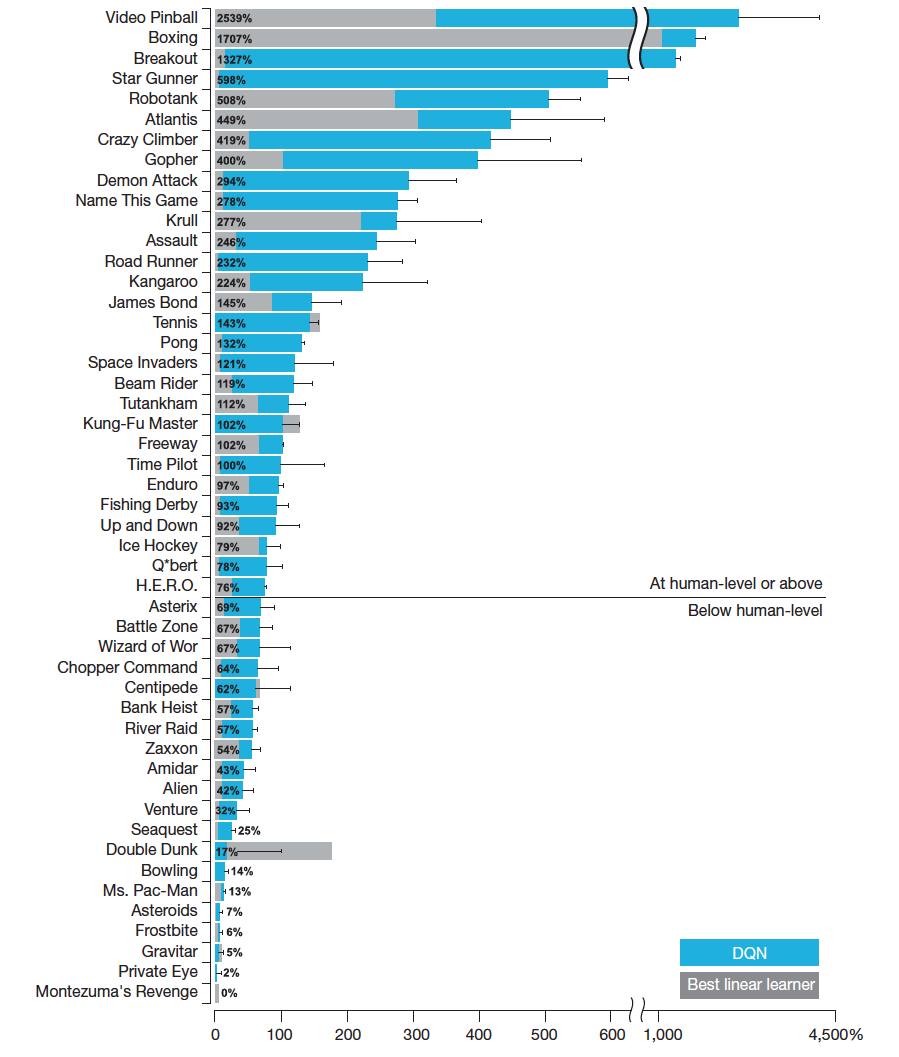
\includegraphics[width=0.7\linewidth]{imagenes/atari.png}
\caption{Juegos de Atari donde un algoritmo de Machine Learning supera a humanos. Fuente:~\cite{mnih-dqn-2015}}
\label{fig:atari}
\end{figure}

En la memoria nos centraremos en el Machine Learning y pondremos énfasis en los tipos que existen y qué algoritmos hay disponibles. Además, describiremos un nuevo método basado en teoría de grafos, y lo compararemos con otros algoritmos clásicos, desarrollando una aplicación que permita analizar conjuntos de datos y comparar entre distintos algoritmos. Por último, usaremos la aplicación para analizar un conjunto de datos.\\

El proyecto tiene los siguientes objetivos:

\begin{enumerate}
\item Introducir qué es el Machine Learning, qué tipos de Machine Learning existen según el tipo de aprendizaje, qué problemas se pueden resolver aplicándolo y familiarizarse con algunos de los algoritmos clásicos.

\item Introducir los conceptos básicos de teoría de grafos, como algunas medidas de redes complejas.

\item Dar a conocer nuevos algoritmos de Machine Learning basados en teoría de grafos, conocidos como redes parenclíticas.

\item Desarrollar una aplicación que automatice el proceso del aprendizaje según distintos algoritmos de Machine Learning (clásicos y basados en teoría de grafos).

\item Analizar una base de datos y comparar los resultados de los distintos algoritmos de Machine Learning.
\end{enumerate}

La memoria está estructurada de la siguiente forma:\\

En el Capítulo~\ref{cap:ml} se introduce el concepto de Machine Learning, qué tipos hay según el aprendizaje y qué tareas permite resolver, así como algunos de los algoritmos existentes según el tipo de aprendizaje.\\

En el Capítulo~\ref{cap:redes_parencliticas}, se introducen brevemente la teoría de grafos, así como un nuevo algoritmo de Machine Learning basado en grafos, las redes parenclíticas.\\

En el Capítulo~\ref{cap:diseño}, se presenta el desarrollo de una aplicación que permita analizar una base de datos utilizando distintos algoritmos de Machine Learning, y compararlos entre ellos.\\

En el Capítulo~\ref{cap:aplicacion}, se analiza una base de datos usando distintos algoritmos de Machine Learning, y una comparación entre ellos.\\

En el Capítulo~\ref{cap:conclusiones}, se presentan las conclusiones y el trabajo futuro. 


%En la actualidad los seres humanos somos unos grandes generadores de datos: al visitar una página web nuestros hábitos de navegación (tipo de ordenador utilizado, navegador, país, hora, etc) quedan almacenados en los servidores de la página web; al realizar una transacción bancaria, nuestro banco guarda datos acerca del cajero utilizado, a qué hora se ha realizado, desde qué país, etc. Éstos son algunos de los lugares donde son recogidos nuestros datos, aunque existen infinidad de ellos.\\

%El objetivo no es almacenar únicamente los datos, sino obtener valor de ellos: en el caso de la página web, se usarán los datos para obtener anuncios o compras (si es una tienda) personalizados, o bloquear tráfico, en caso de que se estuviera produciendo un ataque hacia la página web. En el caso del banco, podría usar los datos para para ofrecer productos personalizados o bloquear transacciones que no se adecuen al comportamiento de un usuario.\\

%Para lograr ésto, se necesitan algoritmos que permitan a los ordenadores ``aprender'' a partir de un conjunto de datos de entrada, para posteriormente inferir sobre nuevos datos. De ésto se encarga el Machine Learning o Aprendizaje Automático.\\

%A lo largo de la memoria veremos qué es el machine learning, qué tipos hay según el tipo de aprendizaje y qué problemas se pueden resolver usándolo, y los algoritmos de machine learning más utilizados.\\

%También veremos otros algoritmos más novedosos: las redes parenclíticas, basadas en teoría de grafos.\\

%Con todo ésto, desarrollaremos una aplicación web para analizar distintos conjuntos de datos usando algoritmos clásicos de machine learning y redes parenclíticas y poder comparar entre ambos algoritmos.\\

%Por último, utilizaremos la aplicación para la detección de tumores en cáncer de mama.  
\chapter{Introducción al Machine Learning}

El Machine Learning o Aprendizaje Automático es la rama de las Ciencias de la Computación, y en particular, de la Inteligencia de la Artificial que se encarga del reconocimiento de patrones y de la teoría computacional del aprendizaje. El machine learning se basa en la construcción de modelos que permitan aprender y hacer predicciones sobre unos datos, de forma automática, es decir, sin intervención humana.\\

El machine learning permite resolver infinidad de problemas que se pueden clasificar de la siguiente manera:

\begin{itemize}
	\item Clasificación: las entradas son divididas entre dos o más clases y el modelo debe aprender a asignar a cada entrada una de las clases.\\
	
	
	Un ejemplo clásico de problema de clasificación es el filtro de spam: el modelo debe ser capaz de identificar un correo electrónico como ``spam'' o ``no spam'', es decir, éstas serán las clases en las que se deberán dividir las entradas (por ejemplo, número de apariciones o frecuencia de distintas palabras en el correo) para identificar el spam.
	
	\item Regresión: las salidas son continuas. En contraposición con la clasificación la regresión tiene una salida continua, es decir, puede tomar todos los valores reales o un intervalo de ellos.\\
	
	Por ejemplo, el valor de las acciones de una determinada empresa a lo largo del tiempo puede ser un ejemplo de regresión, ya que el valor de las acciones pueden tomar cualquier valor en el intervalo $[0, \infty)$.
	
	\item Clustering: un conjunto de entrada se divide en grupos (los grupos no están fijados de antemano).
	
	Un ejemplo clásico es la segmentación del mercado, es decir, encontrar grupos con similares características de una población para ofrecer ofertas personalizadas.
	
	\item Reducción de dimensionalidad: simplifica las entradas por medio de una función a un espacio de dimensión inferior.    
\end{itemize}

En el machine learning puede clasificarse por tipo de aprendizaje:

\begin{itemize}
	\item Aprendizaje supervisado: consiste en construir un modelo a partir de un conjunto de entrenamiento que contiene los datos de entrada y la salida (o etiqueta) esperada. El algoritmo produce un modelo para inferir la salida de nuevos ejemplos.
	
	En este tipo de aprendizaje se incluye la tarea de clasificación y la regresión.
	
	\item Aprendizaje no supervisado: en este caso no existen etiquetas predefinidas de antemano, y se trata de encontrar una función que describa la estructura oculta de los datos.\\
	
	En este tipo de aprendizaje se incluye el clustering.
	
	\item Aprendizaje por refuerzo: un ordenador interactúa con un entorno dinámico para conseguir una determinada, sin que un nadie le diga como de lejos está de conseguirla.  
\end{itemize}

\section{Aprendizaje supervisado}

En el aprendizaje supervisado existe un conjunto de entrenamiento que consiste en un conjunto de datos de entrada junto con su correspondiente salida, que es la respuesta que un algoritmo de machine learning debería producir para esa entrada. Normalmente se representa como $(\mathbf{x}, \mathbf{y})$, donde $x_i$ son las entradas, y $y_i$ son las salidas.\\

Una característica importante de los algoritmos de machine learning es la capacidad de generalización: el algoritmo debería de producir salidas sensatas para entradas que no se introdujeron en el entrenamiento. También es importante que el algoritmo pueda tratar con el ruido, es decir, con las imprecisiones que se  obtienen al medir cualquier variable del mundo real.\\

Dentro de este tipo de aprendizaje tenemos varios tipos de problemas, entre los que se encuentran la clasificación y la regresión.

\paragraph{Clasificación}
El problema de clasificación consiste en tomar las entradas y decidir en cuál de las $n$ clases pertenece cada entrada, basado en el entrenamiento con ejemplares de cada clase. Un punto clave en el problema de clasificación es que es discreto, es decir, cada ejemplo pertenece a una sola de las clases y el conjunto de clases cubre por completo el espacio de salida.

\begin{ejemplo}
Consideremos la clasificación de un correo electrónico como ``spam'' o ``no spam''. En este caso el conjunto de clases vendría dado por $C = \{ \text{spam}, \text{no spam} \}$. Las entradas podrían venir dadas, por ejemplo, por la frecuencia de aparición de distintas palabras claves del correo electrónico. 
\end{ejemplo}

\paragraph{Regresión}
El problema de regresión consiste en obtener un valor de salida a partir de las entradas. En contraposición con el problema de clasificación, las salidas toman valores sobre un intervalo continuo.

\begin{ejemplo}
Supongamos que queremos estimar el valor de las acciones de una determinada empresa a partir de una serie de variables como el número de empleados, los ingresos, etc. En este caso estamos ante un problema de regresión ya que la variable salida (valor de las acciones) toma un valor continuo en el intervalo $[0,\infty)$.  
\end{ejemplo}

\subparagraph{Regresión lineal}
La regresión lineal viene dada por

\begin{equation}
y_i = \sum_{i=1}^{n} \alpha_i x_i + \alpha_0
\end{equation}

donde $y_i$ es la variable salida y $x_i$ es la variable de entrada.\\

El método de mínimos cuadrados nos garantiza que los parámetros $\alpha_i$ que minimizan el error cuadrático vienen dados por

\begin{equation}
\mathbf{\alpha} = (\mathbf{X}^T \mathbf{X})^{-1} \mathbf{X}^T \mathbf{y}.
\end{equation}

En el caso bidimensional el modelo viene dado por

\begin{equation}
y = \alpha_1 x + \alpha_0
\end{equation}

Se tiene que $\alpha_0$ y $\alpha_1$ vienen dados por este sistema de ecuaciones lineales:

\begin{equation}
\begin{cases}
\begin{array}{ccccc}
\left(\sum_{i=1}^{n} x_i^2\right) \alpha_1 & + & \left(\sum_{i=1}^{n} x_i\right) \alpha_0 & = & \sum_{i=1}^{n} x_i y_i \\
 \left(\sum_{i=1}^{n} x_i\right) \alpha_1 & + & n \alpha_0 & = & \sum_{i=1}^{n} y_i
\end{array}
\end{cases}
\end{equation}

\begin{ejemplo}
	Supongamos que disponemos de los datos de la Tabla~\ref{tbl:regresion_lineal} y queremos ajustar un modelo lineal de la forma $y = \alpha_1 x + \alpha_0$.\\
	
	De acuerdo a lo anterior,
	
	\begin{equation*}
	\begin{cases}
	\begin{array}{ccccc}
	92 \alpha_1 & + & 20 \alpha_0 & = & 25 \\
	20 \alpha_1 & + &  8 \alpha_0 & = & 37
	\end{array}
	\end{cases}
	\end{equation*}
	
	Resolviendo el sistema lineal, se tiene que,
	
	\begin{eqnarray*}
	\alpha_1 \approx -1.607 \\
	\alpha_0 \approx  8.642
	\end{eqnarray*}
	
	Por tanto, $y = -1.607x + 8.642$.
	
	Si quisiéramos predecir el valor para $x=7$, tendríamos que $y = -1.607\cdot 7 + 8.642 = -2.607$.
	
	\begin{table}[htbp!]
		\centering
		\caption{Datos para regresión lineal}
		\label{tbl:regresion_lineal}
		\begin{tabular}{@{}lllllllll@{}}
			\toprule
			$x$ & -1 & 0 & 1 & 2 & 3 & 4 & 5 & 6  \\ \midrule
			$y$ & 10 & 9 & 7 & 5 & 4 & 3 & 0 & -1 \\ \bottomrule
		\end{tabular}
	\end{table}
	
\end{ejemplo}

Este método permite ajustar modelos que, en principio, no son lineales como, por ejemplo, 

\[ y = ax^m \]

Este modelo no puede ajustarse como regresión lineal, pero se pueden linealizar las variables $x$, $y$ para convertirlo en un modelo lineal.\\

Tomando logaritmos a ambos lados de la igualdad,

\[ \log y = \log(ax^m)  = \log a + m \log x \]

Haciendo $Y = \log y$, $X = \log x$, $\alpha_1 = \log a$ y $m = \alpha_0$, tenemos un modelo lineal.\\

En la Tabla~\ref{tbl:linealizacion} se pueden encontrar cómo linealizar distintos modelos.

\begin{table}[htbp!]
	\centering
	\caption{Linealización de distintos modelos}
	\label{tbl:linealizacion}
	\begin{tabular}{@{}ccc@{}}
		\toprule
		$y = f(x)$                             & \begin{tabular}[c]{@{}c@{}}Forma linealizada\\ $y = \alpha_1 x + \alpha_0$\end{tabular} & \begin{tabular}[c]{@{}c@{}}Cambio de variables\\ y constantes\end{tabular} \\ \midrule
		$y = \dfrac{\alpha_1}{x} + \alpha_0$   & $y = \alpha_1 \dfrac{1}{x} + \alpha_0$                                                  & $X=\dfrac{1}{x}$; $Y=y$                                                    \\
		$y = \dfrac{1}{\alpha_1 x + \alpha_0}$ & $\dfrac{1}{y} = \alpha_1 x + \alpha_0$                                                  & $Y=\dfrac{1}{y}$; $X=x$                                                    \\
		$y = \alpha_1 \log x + \alpha_0$       & $y = \alpha_1 \log x + \alpha_0$                                                        & $Y = y$; $X = \log x$                                                      \\
		$y = \alpha_1 e^{\alpha_0 x}$          & $\log y = \log \alpha_1 + \alpha_2 \log x$                                              & $Y = \log y$; $X = \log x$; $\alpha_1 = \log \alpha_1$                     \\
		$y = (\alpha_0 + \alpha_1 x)^2$        & $\sqrt{y} = \alpha_0 + \alpha_1 x$                                                      & $Y = \sqrt{y}$; $X=x$                                                      \\ \bottomrule
	\end{tabular}
\end{table}  

\subsection{El proceso de Machine Learning}

El proceso general para resolver un problema usando aprendizaje supervisado consiste en los siguientes pasos:

\begin{enumerate}
	\item Obtención de datos y preparación: consiste en obtener y preparar los datos que se usarán para obtener un modelo de machine learning adecuado para los datos. Consiste en obtener unos datos que sean relevantes, tarea que es difícil cuando se dispone de una cantidad de datos muy grande y que contiene outliers y datos faltantes.
	
	\item Selección de características: consiste en la identificación de características que sean más útiles para el problema en cuestión.
	
	\item Elección del algoritmo: dado el conjunto de datos, consiste en elegir uno o varios algoritmos adecuados que permita resolver el problema de manera satisfactoria.
	
	\item Selección del modelo y sus parámetros: la mayoría de los algoritmos de Machine Learning tienen parámetros que deben ser fijados manualmente, o que requieren experimentación para obtener valores adecuados.
	
	\item Entrenamiento: dado el conjunto de datos, el algoritmo y los parámetros, el entrenamiento deberá construir un modelo a partir de los datos para predecir las salidas de nuevos datos.
	
	\item Evaluación: antes de que el sistema sea desplegado, necesita ser probado y evaluado con datos con los que no ha sido entrenado. A veces, incluye una comparación con expertos humanos en el campo y la selección de métricas apropiadas para esa comparación.    
\end{enumerate}

De los 6 puntos anteriores, nos centraremos en la elección del algoritmo. De entre todos los algoritmos entraremos en detalle de las redes neuronales, los Support Vector Machine (SVM) y los árboles de decisión. 

\subsection{Redes neuronales}

Las redes neuronales fueron propuestas en 1943 por McCulloch y Pitts.

\subsection{Support Vector Machine}

\subsection{Árboles de decisión}

\section{Aprendizaje no supervisado}

\section{Aprendizaje por refuerzo}


\chapter{Redes parenclíticas}

\begin{figure}[htbp!]
	\label{fig:redesparencliticas}
	\begin{center}
		\resizebox{\textwidth}{!}{%
			\redesparencliticas
		}
	\end{center}
	\caption{Esquema del aprendizaje por refuerzo}
\end{figure}
\chapter{Diseño de la aplicación}

\section{Tecnología utilizada}
\chapter[Aplicación análisis de datos de cáncer de mama]{Aplicación análisis de datos de cáncer de mama}

En este capítulo utilizaremos la aplicación descrita en el Capítulo~\ref{cap:diseño} para aplicarla a la detección de tumores en cáncer de mama.

\section{Datos utilizados}

El conjunto de datos ha sido obtenido de~\cite{cancer}. Consta de 699 observaciones y 10 variables (más la variable de clasificación). Éstas son:

\begin{enumerate}
	\item Código de la muestra
	\item Espesor
	\item Uniformidad del tamaño celular
	\item Uniformidad de la forma celular
	\item Adhesión marginal
	\item Tamaño de las células epiteliales
	\item Bare nuclei
	\item Cromatina
	\item Normal Nucleoli
	\item Mitosis
	\item Clase (B = beningno; M = maligno)
\end{enumerate}

Todas las variables toman valores numéricos entre 1 y 10, excepto el número de muestra.\\

Puesto que esta variable no aporta nada, la eliminamos, dejando 10 variables (9 + variable de clasificación).\\

Un subconjunto de los datos se puede ver en la Figura~\ref{fig:datos_cancer}.\\

\begin{figure}[tbph!]
\centering
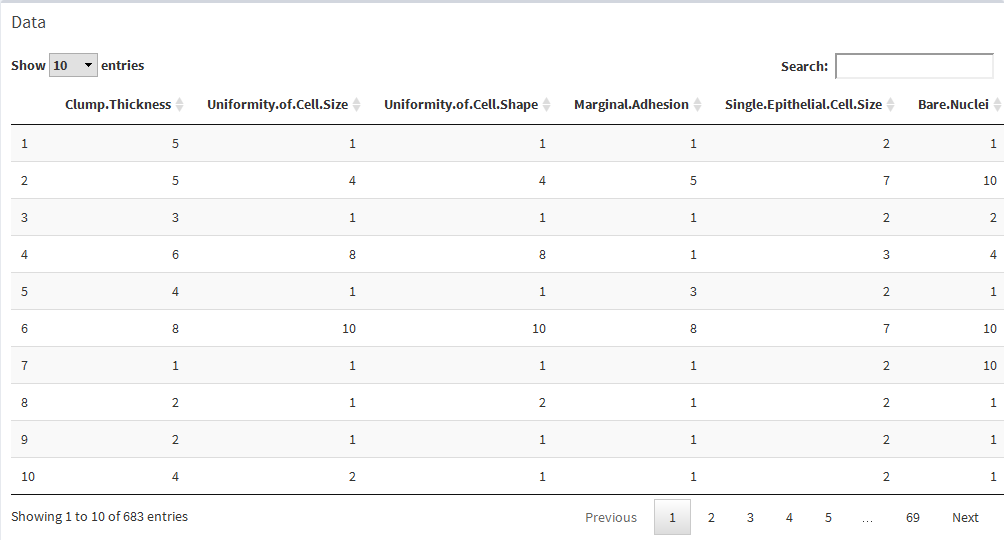
\includegraphics[width=0.6\linewidth]{imagenes/cancer/datos.png}
\caption{Subconjunto de los datos de cáncer de mama}
\label{fig:datos_cancer}
\end{figure}

Con la aplicación podemos ver cuál es la distribución de cada una de las variables. Por ejemplo, en el caso del espesor la distribución por clase de tumor se puede ver en la Figura~\ref{fig:thickness}.\\

\begin{figure}[tbph!]
	\centering
	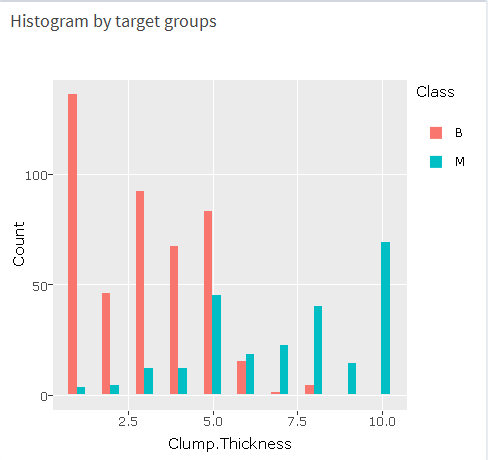
\includegraphics[width=0.5\linewidth]{imagenes/cancer/thickness.png}
	\caption{Distribución del espesor por clase de tumor}
	\label{fig:thickness}
\end{figure}

Se puede observar que la presencia de un espesor menor está presente en tumores benignos, y a medida que el espesor es mayor se producen más tumores malignos.\\

\begin{figure}[htbp!]
	\begin{center}
		\begin{subfigure}[t]{\textwidth}
			\centering
			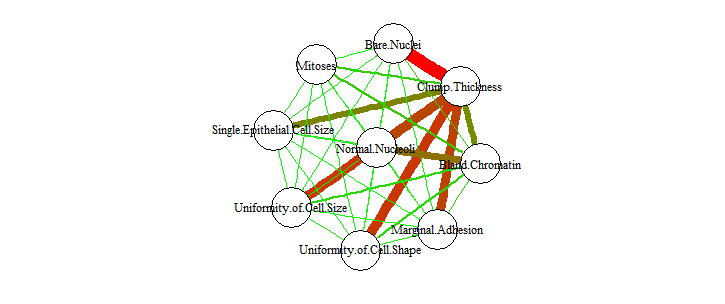
\includegraphics[height=7.5cm]{imagenes/cancer/1.png}
			\caption{Red parenclítica de la observación 1}
		\end{subfigure}
		\begin{subfigure}[t]{\textwidth}
			\centering
			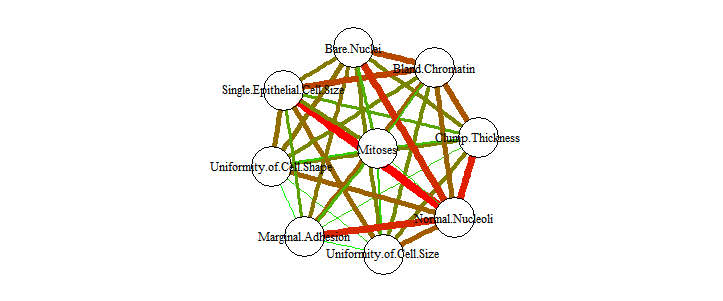
\includegraphics[height=7.5cm]{imagenes/cancer/2.png}
			\caption{Red parenclítica de la observación 2}
		\end{subfigure}
		
	\end{center}
	\caption{Redes parenclíticas con modelo de regresión lineal}
	\label{fig:cancer_par}
\end{figure}
 
En la Figura~\ref{fig:cancer_par} se pueden observar las redes parenclíticas de las dos primeras observaciones obtenidas con el modelo lineal.\\

Podemos ver si existen diferencias entre las redes parenclíticas de las observaciones con tumores benignos y malignos. La Figura~\ref{fig:cancer_diferencias} muestra cuatro observaciones de cada clase de tumor.\\

\begin{figure}[htbp!]
	\begin{center}
		\begin{subfigure}[t]{0.2\textwidth}
			\centering
			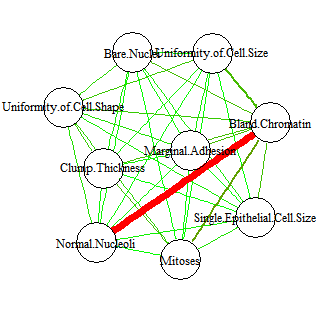
\includegraphics[height=3cm]{imagenes/cancer/b1.png}
			\caption{Obs. 8}
		\end{subfigure}
		\begin{subfigure}[t]{0.2\textwidth}
			\centering
			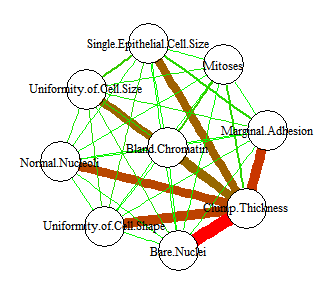
\includegraphics[height=3cm]{imagenes/cancer/b2.png}
			\caption{Obs. 26}
		\end{subfigure}
		\begin{subfigure}[t]{0.2\textwidth}
			\centering
			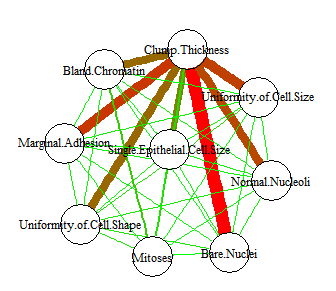
\includegraphics[height=3cm]{imagenes/cancer/b3.png}
			\caption{Obs. 34}
		\end{subfigure}
		\begin{subfigure}[t]{0.2\textwidth}
			\centering
			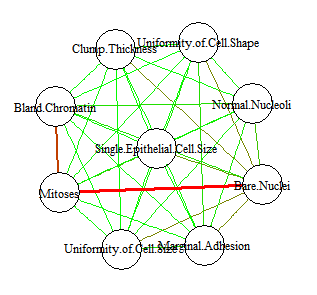
\includegraphics[height=3cm]{imagenes/cancer/b4.png}
			\caption{Obs. 60}
		\end{subfigure}	
		
		\begin{subfigure}[t]{0.2\textwidth}
			\centering
			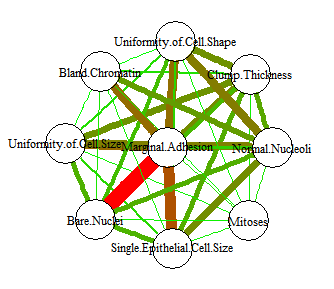
\includegraphics[height=3cm]{imagenes/cancer/m1.png}
			\caption{Obs. 41}
		\end{subfigure}
		\begin{subfigure}[t]{0.2\textwidth}
			\centering
			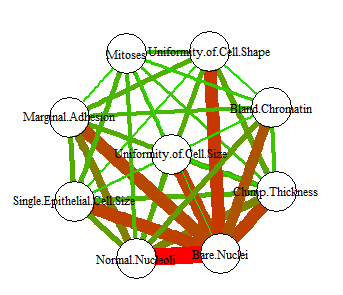
\includegraphics[height=3cm]{imagenes/cancer/m2.png}
			\caption{Obs. 43}
		\end{subfigure}
		\begin{subfigure}[t]{0.2\textwidth}
			\centering
			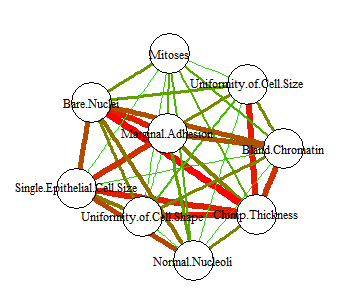
\includegraphics[height=3cm]{imagenes/cancer/m3.png}
			\caption{Obs. 50}
		\end{subfigure}
		\begin{subfigure}[t]{0.2\textwidth}
			\centering
			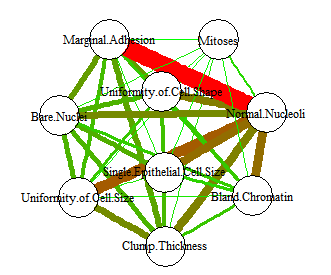
\includegraphics[height=3cm]{imagenes/cancer/m4.png}
			\caption{Obs. 51}
		\end{subfigure}		
	\end{center}
	\caption[Redes parenclíticas por clase de tumor con modelo de regresión lineal]{Redes parenclíticas por clase de tumor con modelo de regresión lineal. En la primera fila se muestran las observaciones con tumor benigno y, en la segunda, con tumor maligno}
	\label{fig:cancer_diferencias}
\end{figure}

Se puede observar que en el caso de las observaciones con tumor benigno existe un menor peso en las aristas (color verde de las aristas), y en las observaciones con tumor maligno existe un mayor entre las aristas (color rojo de las aristas).\\

Puesto que disponemos de varios modelos de regresión, puede que el modelo lineal no sea el más indicado, por lo que calculamos la regresión para cada uno de los modelos de regresión (lineal, exponencial, cuadrática y recíproca), junto con la de los modelos de machine learning clásicos (árboles de decisión, Support vector Machine y redes neuronales), y calculamos la curva ROC de cada clasificador (Figura~\ref{fig:roc_cancer}).\\

\begin{figure}[tbph!]
	\centering
	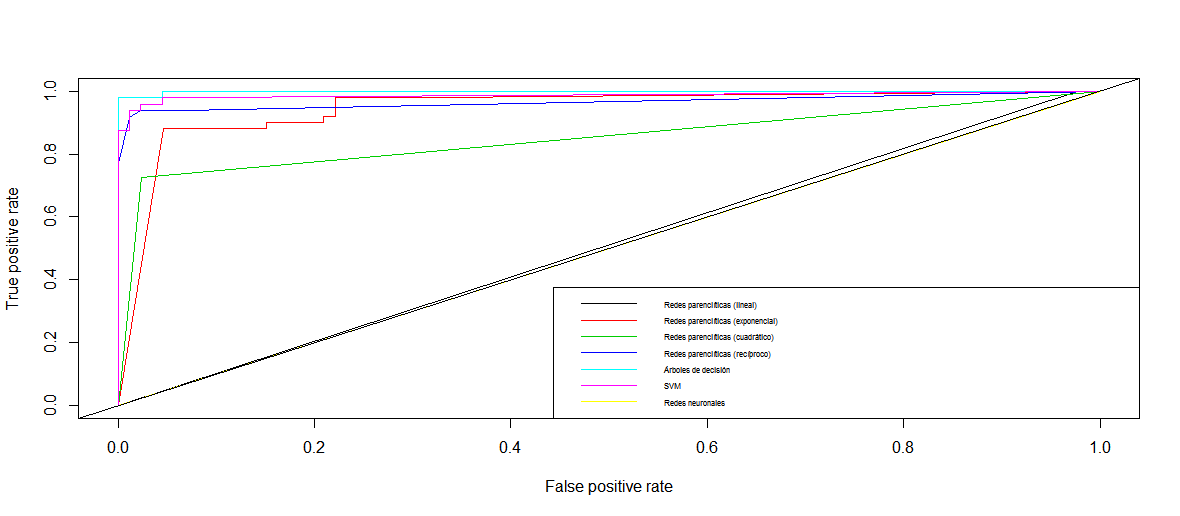
\includegraphics[width=0.9\linewidth]{imagenes/cancer/ROC_cancer.png}
	\caption{Curvas ROC}
	\label{fig:roc_cancer}
\end{figure}

Se puede observar que el mejor clasificador por redes parenclíticas es el obtenido con el modelo de regresión recíproco, seguido del exponencial y el cuadrático. El peor clasificador es el lineal. Respecto a los algoritmos clásicos de machine learning, el mejor clasificador son los árboles de decisión seguido de los Support Vector Machine y de las redes neuronales.\\

Sobre todos los clasificadores, el mejor son los árboles de decisión, seguido de los Support Vector Machine y las redes parenclíticas con modelo recíproco.\\
 
Puesto que el mejor modelo de redes parenclíticas es el modelo recíproco, veamos si existen diferencias entre las redes parenclíticas según la clase de tumor (Figura~\ref{fig:cancer_rec}).\\

\begin{figure}[htbp!]
	\begin{center}
		\begin{subfigure}[t]{0.25\textwidth}
			\centering
			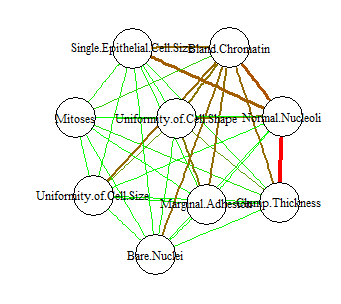
\includegraphics[height=3cm]{imagenes/cancer/b1_reciproco.png}
			\caption{Obs. 8}
		\end{subfigure}
		\begin{subfigure}[t]{0.25\textwidth}
			\centering
			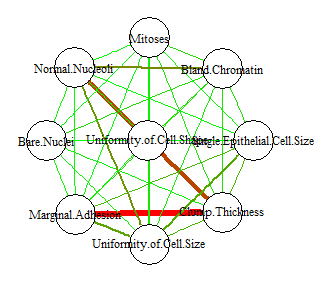
\includegraphics[height=3cm]{imagenes/cancer/b2_reciproco.png}
			\caption{Obs. 26}
		\end{subfigure}
		\begin{subfigure}[t]{0.25\textwidth}
			\centering
			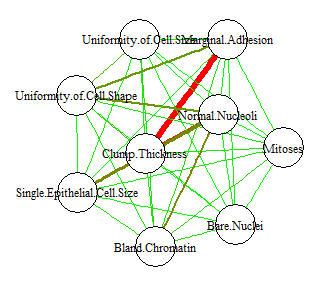
\includegraphics[height=3cm]{imagenes/cancer/b3_reciproco.png}
			\caption{Obs. 34}
		\end{subfigure}
		
		\begin{subfigure}[t]{0.25\textwidth}
			\centering
			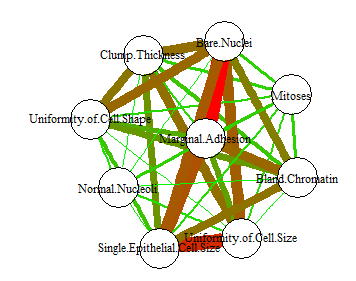
\includegraphics[height=3cm]{imagenes/cancer/m1_reciproco.png}
			\caption{Obs. 41}
		\end{subfigure}
		\begin{subfigure}[t]{0.25\textwidth}
			\centering
			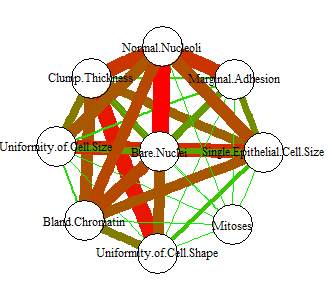
\includegraphics[height=3cm]{imagenes/cancer/m2_reciproco.png}
			\caption{Obs. 43}
		\end{subfigure}
		\begin{subfigure}[t]{0.25\textwidth}
			\centering
			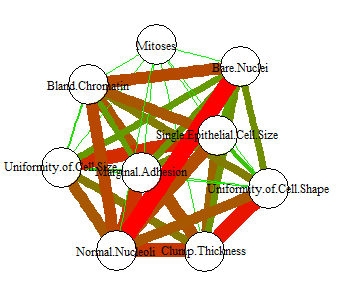
\includegraphics[height=3cm]{imagenes/cancer/m3_reciproco.png}
			\caption{Obs. 50}
		\end{subfigure}
	\end{center}
	\caption[Redes parenclíticas por clase de tumor con modelo de regresión recíproco]{Redes parenclíticas por clase de tumor con modelo de regresión recíproco. En la primera fila se muestran las observaciones con tumor benigno y, en la segunda, con tumor maligno}
	\label{fig:cancer_rec}
\end{figure}

Se puede observar que los pacientes con tumores malignos tienen una cantidad de aristas con mayor peso (representadas con el color rojo), mientras que en el caso de los pacientes con tumores benignos se da el caso contrario, existe una cantidad mayor de aristas con peso pequeño (representado en color verde). Así pues, parece que existen diferencias según el tipo de tumor (benigno y maligno) atendiendo solamente a la estructura de la red parenclítica.


\section{Umbralización de las redes parenclíticas}

Hasta ahora, las redes parenclíticas usadas eran grafos completos, es decir, que existe una arista entre cada par de variables. Esto implica que algunas medidas no son adecuadas sobre grafos completos, ya que siempre se obtiene el mismo valor de la medida. Para solventar este problema, normalizaremos (en el intervalo $[0,1]$) los pesos de las aristas de cada una de las redes parenclíticas, y eliminaremos las aristas cuyos pesos sean menores o iguales que un valor $x \in [0,1]$, y realizaremos la clasificación de igual manera que en los casos anteriores (Figura~\ref{fig:ejemploumbralizacion}).


\begin{figure}[tbph!]
	\centering
	\ejemploumbralizacion
	\caption{Ejemplo de umbralización de una red parenclítica. En primer lugar, se normaliza las aristas de la red en el intervalo $[0,1]$, y por cada $x \in [0,1]$ se eliminan las aristas menores o iguales que $x$}
	\label{fig:ejemploumbralizacion}
\end{figure}

Si aplicamos este procedimiento a los datos de cáncer de mama para cada uno de los cuatro tipos de regresión (lineal, exponencial, cuadrático y recíproco), con paso de umbralización $0.01$, atendiendo a la tasa de aciertos, los resultados se muestran en la Figura~\ref{fig:umbralizacion}.\\

\begin{figure}[tbph!]
	\centering
	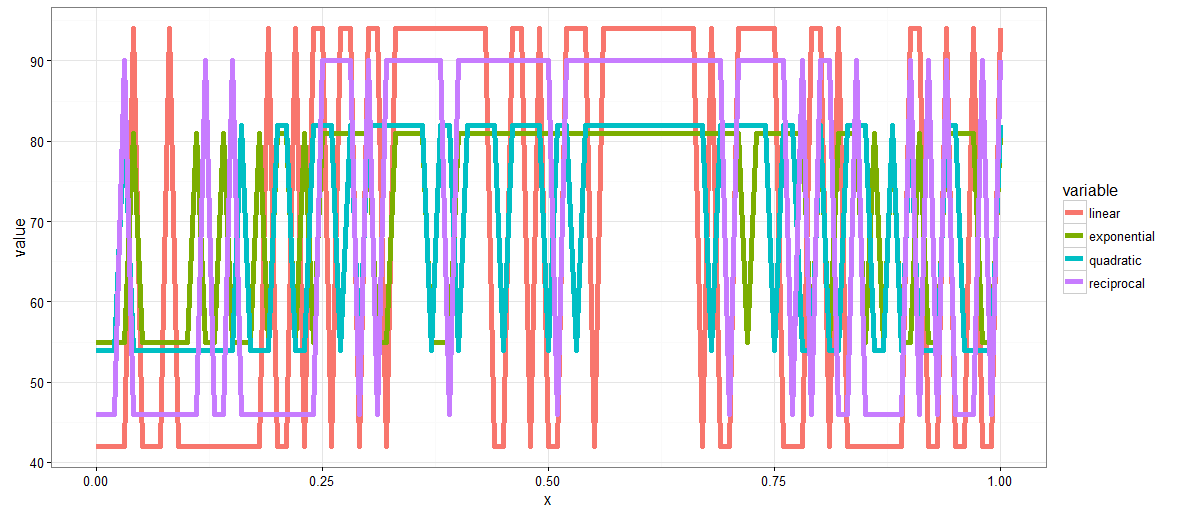
\includegraphics[width=1\linewidth]{imagenes/cancer/umbralizacion.png}
	\caption{Porcentaje de acierto por cada tipo de método de regresión, usando la umbralización de las redes parenclíticas}
	\label{fig:umbralizacion}
\end{figure}

Se puede observar que el método de umbralización mejora el porcentaje de clasificación de cada uno de los métodos de regresión. En especial, mejora el método de regresión lineal, que con las redes parenclíticas con grafos completos apenas superaba el 50\% de acierto, con el método de umbralización supera el 90\%. En los otros métodos de regresión, se produce el mismo efecto, pero la mejora es inferior que en el caso del método de regresión lineal. Notar que se producen fuertes variaciones en la tasa de acierto para valores muy cercanos de la umbralización. Esto puede ser debido a que al realizar el entrenamiento con redes neuronales, ésta se queda atrapada en un mínimo local, lo que produce una baja tasa de aciertos. El valor óptimo $x$ para los cuatro métodos están el intervalo $[0.55, 0.65]$, ya que es estos valores maximizan la tasa de acierto.\\


\chapter{Conclusiones}\label{cap:conclusiones}

Durante la memoria hemos visto qué es el Machine Learning, qué tipos existen según el tipo de aprendizaje y qué tareas permiten resolver. Para cada uno de los tipos de aprendizaje hemos visto qué es lo que caracteriza a cada uno, qué tareas se pueden resolver y algunos de los algoritmos que se pueden aplicar.\\

Hemos visto que es posible usar la teoría de grafos para desarrollar un nuevo algoritmo de Machine Learning para realizar la tarea de clasificación binaria. Hemos visto cómo generalizar el método a una clasificación multiclase, cómo aplicar distintos métodos de regresión para realizar la clasificación.\\

Hemos desarrollado una aplicación que analiza y compara un conjunto de datos según distintos algoritmos de Machine Learning.\\

Por último, hemos aplicado la aplicación al diagnóstico de tumores de cáncer de mama, obteniendo grandes resultados, aunque sin llegar al nivel de los algoritmos clásicos. Además, hemos visto que umbralizando las redes parenclíticas es posible obtener mejores resultados que con los grafos completos.
   
\section{Mejoras y futuro trabajo}

\begin{itemize}
	\item Optimización de los algoritmos de redes parenclíticas: se deben optimizar los algoritmos de aprendizaje de redes parenclíticas para minimizar la cantidad de memoria empleada y el tiempo de procesamiento para conjuntos de datos muy grandes.
	 
	\item Mejora en visualización de la aplicación: mejora de la interfaz gráfica para conseguir una mejor experiencia de usuario, con la consiguiente migración a HTML 5 y CSS 3 ``nativo''.
	
	\item Nuevos métodos de regresión: adición de nuevos métodos de regresión como la regresión logística o la no lineal, o incluso, algoritmos de Machine Learning que permitan la tarea de regresión, como SVM o redes neuronales.
	
	\item Persistencia de las redes parenclíticas en bases de datos de grafos: almacenamiento persistente de las redes parenclíticas en bases de datos de grafos como OrientDB~\cite{orientdb}, Titan~\cite{titan} o Neo4j~\cite{neo4j} para realizar futuros procesamientos o visualizaciones.
\end{itemize}

\appendix
\input{anexos/manual_instalación}

\backmatter
\nocite{*}
\bibliographystyle{plain}
\bibliography{bibliografia/bibliografia}
\nobibintoc

\end{document}